%!TEX root = ../hausarbeit.tex
%!TEX spellcheck = de_DE
% Hauptmenuepunkt
\section{Einleitung}\label{Einleitung}
%\addcontentsline{toc}{section}{Einleitung}
Die Lebensgefährtin des Autors ist Leitung der Kinderkrippe Tannenweg in Ingelheim. Während ihres Studiums zum Bachelor of Arts im Fachbereich "{}Bildungs- und Sozialmanagement"{} entwickelte sie im Rahmen einer Projektarbeit ein Übergabebuch zur Organisation innerhalb ihrer Krippengruppe. 

Da der Autor Student der Sozialinformatik an der Hochschule Fulda ist, trat die Leitung an Ihn heran, um das bislang genutzte Übergabeheft in eine digitale Form zu überführen und den Prozess somit weiter zu verbessern.

In dieser Hausarbeit soll nun zunächst analysiert werden, was  Qualitätsmanagement ist und ob es sinnvoll in Kindertagesstätten eingesetzt werden kann. Anschließend soll der ursprüngliche Prozess nach QM-Standards analysiert werden, woraufhin Verbesserungsmöglichkeiten und die Einsatzmöglichkeiten der Sozialinformatik aufgezeigt werden. Diese Hausarbeit schließt mit einem persönlichen Fazit zu den behandelten Themenbereichen.

Der Autor ist zur Zeit als System- und Netzwerkadministrator in der Finanzverwaltung Rheinland-Pfalz beim Finanzamt Mainz beschäftigt. Hier ist er Ansprechpartner für die Nutzer im Umgang mit technischen Systemen sowie für Steuerpflichtigen bei der Nutzung der elektronischen Steuererklärung ELSTER. 

Der Autor hat keine fach-technische Ausbildung, sondern ist ausgebildeter Finanzbeamter und wurde aufgrund seiner Kenntnisse im Umgang mit PCs und Technik im Allgemeinen auf eigenen Wunsch in die Administration versetzt worden.

\newpage

\section{Das Unternehmen}

Das behandelte Unternehmen ist die Kinderkrippe "{}Tannenweg"{} in Ingelheim am Rhein. Die Einrichtung ist in kommunaler Trägerschaft, es besteht jedoch ein Kooperationsvertrag mit dem lokalen Pharmaunternehmen Boehringer Ingelheim.

Das Haus verfügt über vier Gruppen mit insgesamt 40 Betreuungsplätzen. In der Einrichtung arbeiten insgesamt sieben pädagogische Fachkräfte und fünf Kinderkrankenschwestern so wie zwei hauswirtschaftliche Kräfte.

Die Kinderkrippe ist täglich von 6:45 Uhr bis 18:00 Uhr bzw. freitags bis 17:00 Uhr geöffnet. Folglich besteht ein System aus Früh- und Spätschicht der Vollzeitkräfte, um die langen Öffnungszeiten abzudecken.

Im Rahmen der fortschreitenden Digitalisierung ist geplant, in naher Zukunft ein flächendeckendes internes WLAN in der Kinderkrippe aufzubauen und die Gruppen mit Tablets auszustatten.

\subsection{Der Prozess}

Die Weitergabe von Informationen zwischen den Schichtsystemen ist ein zentrales Thema in der Kinderkrippe.
Zur Abstimmung der Informationen und zur Dokumentation von Vorkommnissen im Betreuungsalltag wird in den einzelnen Gruppen ein Übergabeheft geführt. In diesem Heft werden die kindbezogenen Informationen über den Tag dokumentiert. Ist das Kind z.B. während der Frühschicht gefallen, wird dies im Übergabeheft vermerkt, sodass der Spätdienst diese Information bei der Übergabe des Kindes an die Eltern mitteilen kann.

Die Einführung des Heftes wurde durch eine damalige Gruppenkollegin durch eine Projektarbeit im Rahmen Ihres Studiums begleitet. Es zeigte sich eine enorme Verbesserung der Qualität im pädagogischen Arbeitsalltag der Einrichtung.

Das ursprünglich eingeführte Übergabeheft war ein für die Gruppe angeschafftes DinA5-Heft, in dem die entsprechenden Informationen vermerkt wurden. Nach der Verbreitung des Konzeptes auf die anderen Gruppen wurde der Wunsch nach einer Vereinheitlichung und einer Vereinfachung des Konzeptes laut.

Informationen werden zur Zeit im Laufe des Tages auf einem laminierten Papier mit wasserlöslichem Folienschreiber vermerkt. Der Spätdienst reinigt jeden Abend zum Dienstende das Papier, damit der Frühdienst morgens keine Zeit mit Vorbereitungsarbeiten verliert.

Leider läuft der Prozess noch nicht optimal. 
Informationen die der Spätdienst gesammelt hat, werden durch die Reinigung nicht für den Frühdienst des nächsten Tages konserviert. 

%\newpage

\section{QM in Kindertageseinrichtungen}

Qualität beschreibt umgangssprachlich \textquote{die Güte, den Wert oder die Beschaffenheit eines Gutes oder einer Leistung} \citep[][8]{studi14}.
Hier zeigt sich ein Problem des Qualitätsmanagements (QM) in sozialen Einrichtungen wie einer Kindertagesstätte. Schließlich kann die Qualität der Leistung "{}Kinderbetreuung"{} nicht anhand klarer objektiver Maßstäbe gemessen werden. Mehr noch als in z.B. der verarbeitenden Industrie ist Qualität in der sozialen Arbeit eine subjektive Erfahrung. Auch unterliegt sie einem steten Wechsel durch Veränderung der Wertvorstellung des Einzelnen oder der Gesellschaft \citep[vgl.][9]{studi14}.

\textquote{Die Einführung eines Qualitätsmanagementsystems ist eine strategische Entscheidung einer Organisation, die helfen kann, ihre Gesamtleistung zu steigern [...].} \citep[][8]{ISO9001}. Das Qualitätsmanagement nach ISO 9001 geht hier einen anderen Weg. Beschreibt die oben erwähnte Betrachtung von Qualität einen ergebnissorientierten Ansatz, fördert die Norm \textquote{[...] die Umsetzung eines prozessorientierten Ansatzes bei der Entwicklung, Verwirklichung und Verbesserung der Wirksamkeit eines Qualitätsmanagementsystems, um die Kundenzufriedenheit durch Erfüllen der Kundenanforderung zu erhöhen.} \citep[][10]{ISO9001}.

Merchel beobachtet, dass sich Organisationen der sozialen Arbeit nicht gleichmäßig verändern. \textquote{Bemerkenswertes Beharrungsvermögen ist genauso zu registrieren wie die Bereitschaft zum deutlichen Organisationswandel.} \citep[][12]{Merchel2005}. Der Autor führt weiter aus, dass Veränderungsimpulse unter Anderem auch aus Umweltanforderungen entstehen \citep[vgl.][13]{Merchel2005}.

Der  Erwartungsdruck seitens Politik und Öffentlichkeit erfordert von den Kitas enorme Leistungen. \textquote{Die Kitas werden als Allheilmittel gesehen um viele schwerwiegende Probleme zu lösen - von der nachhaltigen Integration zugewanderter Menschen bis hin zur raschen Rückkehr von Eltern in das Erwerbsleben, [...]} \citep[][11]{KitaMana}.
Die Prozessorientierung von Qualitätsmanagementsystemen nach der ISO 9001 ermöglicht es Kindertagesstätten, der Forderung nach der Öffnung für Qualitätsentwicklungsprozesse \citep[vgl.][26]{KitaMana} nachzukommen.

Qualitätsorientiertes Arbeiten ist den Beschäftigten einer Kita jedoch nicht fremd. \textquote{Auch ohne ein implementiertes Qualitätsmanagementsystem (QMS) haben viele Kitas die wesentlichen Kernprozesse des QMS differenziert beschrieben, [...]} \citep[][197]{KitaMana}. Bombosch führt in seinem Aufsatz weiter aus, dass solche Teams in der Regel bereits einen Großteil der Forderungen aus den für Kitas relevanten QMS erfüllen.

Bombosch definiert im folgenden nach Haderlein Qualität im Kita-Bereich als \textquote{[...] all das, was positive Wirkung auf die Entwicklung der Persönlichkeit eines jungen Menschen hat. [...]} \citep[][198]{KitaMana}. Durch diese Definition ist es möglich, die Qualität der Kita zu steigern, in dem Hilfsprozesse, die Auswirkung auf die Umgebung der betreuten Kinder haben, über das Qualitätsmanagementsystem analysiert und verbessert werden

Im folgenden soll nun betrachtet werden, in wie weit der PDCA-Zyklus der ISO 9001 im Qualitätsmanagement einer Kindertagesstätte Anwendung finden kann.

\subsection{PDCA-Zyklus}
PDCA steht für "{}\textit{Plan, Do, Check, Act}"{} oder übersetzt "{}\textit{Planen, Durchführen, Prüfen, Handeln}"{} \citep[vgl.][9]{ISO9001}
\begin{figure}[h]
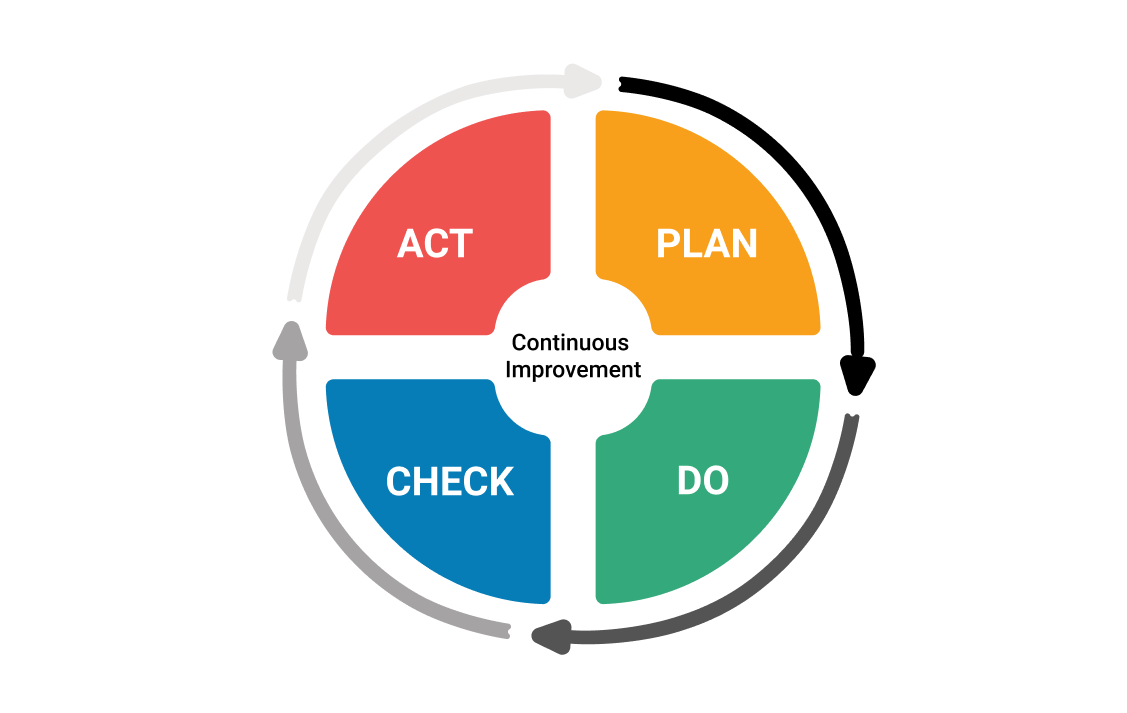
\includegraphics[width=1.0\textwidth]{res/pdca.png}\\
\caption{Darstellung des PDCA-Zyklus \citep[][]{pdca}}
\end{figure}
Gemäß der Norm bedeutet dies:

\blockquote{\begin{itemize}
		\item Planen \\
			Festlegen von Zielen des Systems und der Teilprozesse und Festlegen von Ressourcen, die zum Erzielen von Ergebnissen und Übereinstimmung mit den Kundenanforderungen und den Politiken der Organisation notwendig sind, sowie Ermitteln und Behandeln von Risiken und Chancen;
		\item Durchführen\\
			Umsetzen des Geplanten;
		\item Prüfen\\
			Überwachen und (sofern zutreffend) Messen von Prozessen und den daraus resultierenden Produkten und Dienstleistungen im Hinblick auf Politiken, Ziele, Anforderungen und geplante Tätigkeiten, sowie Berichterstattung über die Ergebnisse;
		\item Handeln\\
			Ergreifen von Maßnahmen zur Verbesserung der Leistung soweit notwendig
	\end{itemize}}\citep[][14]{ISO9001}

Vereinfacht lässt sich, nach Bombosch, PDCA wie folgt zusammenfassen: \textquote{Ich plane etwas, setze es um, überprüfe das Umgesetzte auf seine Bedeutung und Praktikabilität [...] und suche nach Verbesserungspotential.} \citep[][199]{KitaMana}.


Doch was bedeutet dies nun für das eingangs dargestellte Übergabebuch in der Kinderkrippe Tannenweg? Lässt sich der Prozess im Rahmen eines Qualitätsmanagementsystems darstellen? Dies soll im nächsten Kapitel genauer betrachtet werden.

\newpage
\section{Qualitätsmanagement anhand des Prozesses "{}Übergabebuch"{}}

Bombosch berichtet in seinem Fachaufsatz von Erzieherinnen, die von sich überzeugt seien, schon immer nach qualitativen Maßstäben zu arbeiten \citep[vgl.][197]{KitaMana}. 
Dies wirft die Frage auf, ob auch bei der Einführung des Übergabebuches unbewusst die Regeln des Qualitätsmanagements nach ISO 9001 befolgt wurden. Daher soll nun der PDCA-Zyklus auf das Ursprungsproblem der nicht weitergegebenen Informationen angewandt werden. Hierbei soll untersucht werden, ob die bereits durchgeführten Handlungen im Rahmen eines PDCA-Zyklus angebracht gewesen wären.

\subsection{Adressierung des Problems}

Anstoß des Wunsches nach Änderung war eine interne Diskrepanzerfahrung wie von Merchel beschrieben. \textquote{"{}Diskrepanzerfahrungen"{} entstehen bei den Organisationsmitgliedern immer dann, wenn sie eine Spannung zwischen dem vorhandenen Zustand (den vermeintlichen Gegebenheiten) einer Organisation und einem von ihnen als Soll definierten Zustand einer Organisation wahrnehmen und wenn diese Wahrnehmung als so störend empfunden wird, dass die Spannung zu Veränderungswünschen führt} \citep[][19]{Merchel2005}.

Die Diskrepanzerfahrung war die Tatsache, dass Informationen zwischen dem Früh- und Spätdienst verloren gingen. Dies führte seitens der Mitarbeiter auch zu Frust. Der Wunsch der Organisationsmitglieder war, einen Prozess zu schaffen, der Informationen für alle Mitglieder verfügbar machte. 

Auch konnte die Anforderung des Kunden \citep[vgl.][22]{ISO9001} nicht erfüllt werden, da Eltern nur ungenügend über Vorfälle im Kita-Alltag ihres Kindes informiert wurden.

\subsection{PDCA Schritt 1: Planen}
\textquote{Bei Planungen für das Qualitätsmanagementsystem muss die Organisation die in 4.1 genannten Themen und die in 4.2 genannten Anforderungen berücksichtigen sowie die Risiken und Chancen bestimmen, die behandelt werden müssen, [...]}\citep[][23]{ISO9001}.

Als Risiken des Prozesses sind hauptsächlich persönliche Adaptionsprobleme seitens der Organisationsmitglieder zu nennen. Der eingeführte Prozess könnte falsch verstanden und in der Folge nicht korrekt durchgeführt werden. Auch könnten Mitarbeiter generell von Änderungen abgeschreckt werden oder Prozess aus einer persönlichen Abneigung heraus behindern und sabotieren.

Als Chance fällt zunächst ins Auge, dass bei einem korrekt eingeführten Prozess die Informationsweitergabe ungehindert funktionieren könnte. Eltern würden über Vorfälle im Alltag ihrer Kinder informiert, Kollegen des nächsten Tages z.B. über eine geänderte Bringzeit in Kenntnis gesetzt. 

Teil des Abschnittes Planung im Sinne der Norm ist es unter Anderem \textquote{Verbesserung zu erreichen}\citep[][23]{ISO9001}

Die Projektverantwortliche (die Lebensgefährtin des Autors) musste einen Prozess planen, der die Informationsweitergabe vereinfachte um somit sowohl die Kunden- als auch die Mitarbeiterzufriedenheit zu steigern. Sie plante die Implementierung eines Buches, in dem für jeden Tag und jedes Kind Platz wäre um Besonderheiten oder Vorkommnisse zu notieren. Diese sollten am betreffenden Tag in die entsprechende Spalte vermerkt werden.

\subsection{PDCA Schritt 2: Durchführen}

Die in Schritt 1 geplanten Tätigkeiten müssen umgesetzt werden.

Es wurde ein Din-A5 Heft beschafft. Die Projektverantwortliche beschriftete jede Doppelseite mit einer Wochennummer und zeichnete Linien auf die Seiten um Eintragungsmöglichkeiten für die Kinder (Zeilen) und Tage (Spalten) zu erhalten. 

In einer kurzen Einweisung wurden die weiteren Gruppenmitglieder über das Übergabeheft informiert.

\subsection{PDCA Schritt 3: Prüfen}

Wie bereits weiter oben erwähnt, ist es nun an der Zeit zu prüfen, ob die gesetzten Ziele durch die Planung in Schritt 1 und die Durchführung in Schritt 2 Erfolg gebracht haben. Im dargestellten Fall brachte die Maßnahme durchaus den gewünschten Erfolg. Die Informationsweitergabe erfolgte zielgerichtet und flüssig. 

Jedoch wurde von Seiten der Kollegen der Ressourcenverbrauch bemängelt. Jede Gruppe hatte nun ein Heft, welches beschrieben und anschließend weggeworfen wurde. Schließlich waren die Informationen nach kurzer Zeit überholt, eine Archivierung der Bücher erschien als nicht zweckdienlich.

\subsection{PDCA Schritt 4: Handeln}

Gemäß der Norm \citep[vgl.][14]{ISO9001} müssen nach der Prüfung des Prozesses Maßnahmen ergriffen werden, um die in Schritt 3 aufgezeigten Verbesserungsmöglichkeiten zu nutzen und den Prozess zu optimieren. 

Das Übergabebuch wurde überarbeitet. Es wurde ein größeres Blatt Papier entsprechend des erarbeiteten Layouts vorbereitet. Die Spalten für die Tage entfallen, es gibt nun nur noch Zeilen für die einzelnen Kinder.\\
Anschließend wurde das Blatt laminiert.
Es wurden wasserlösliche Folienstifte besorgt und in den Gruppen verteilt. Der jeweilige Frühdienst ist für die Reinigung und Vorbereitung des Blattes für den nächsten Tag zuständig. Somit konnte Nachhaltigkeit erzeugt werden, da nur noch ein einziges Blatt wiederverwendet werden kann.

Es bleibt festzustellen, dass bereits bei der Einführung des Übergabebuch die wesentlichen Regeln des PDCA-Zyklus berücksichtigt wurden. Es soll nun im nächsten Kapitel die Einsatzmöglichkeit der Sozialinformatik aufgezeigt werden, um den Prozess weiterzuentwickeln und neu aufgetretene Schwächen zu kompensieren.

\newpage
\section{Ansatzpunkte der Sozialinformatik}

\textquote{[Komplexe Technologien]...beeinflussen immer die sozialen Systeme, in denen sie eingesetzt werden und werden umgekehrt wiederum von von diesen Systemen adaptiert und beeinflusst} \citep[][24]{kreidenweis2012}.

Aufgrund von Unachtsamkeit kommt es immer wieder vor, dass der Frühdienst das Übergabeblatt reinigt, ohne die Vermerke des Spätdienstes zu bemerken. Somit sind die Informationen zunächst verloren. Dies stellt sich als enormes Problem für die Erreichung der Ziele heraus.

Die Leitung plant daher, den Prozess erneut umzugestalten, um den Informationsfluss zu verbessern und somit die Kunden- und Mitarbeiterzufriedenheit weiter zu erhöhen.

Die Sozialinformatik als Bindeglied zwischen der Informatik und den Mitarbeitenden der sozialen Arbeit kann hier Chancen aufzeigen, um den Prozess mit digitaler Unterstützung zu optimieren. \textquote{Über den Markterfolg sozialer Organisationen werden künftig immer stärker [...] die Verzahnung von Technik und personaler Dienstleistung mit entscheiden}\citep[][90]{kreidenweis2012}.

Da die Leitung der Kinderkrippe Tannenweg plant, die Gruppen mit Tablets und WLAN auszustatten, läge es nahe, eine webbasierte Datenbank einzurichten, in der die einzelnen Teammitglieder die jeweiligen Informationen ablegen könnten. 

Da gerade beim Thema Datenschutz ein hohes Bedürfnis nach Sicherheit besteht, sollen die Informationen selbstverständlich nicht ins Internet geladen werden. Denkbar wäre, ein Network Attached Storage (NAS) oder einen kleinen Server einzurichten, welcher dann über eine Weboberfläche bedient wird.

Am einfachsten ließe sich der Prozess vermutlich mit einer Kalenderanwendung abbilden, in der die einzelnen Teammitglieder jeweils Schreibberechtigung für Ihren Teamkalender haben. Somit wäre auch der Datenschutz zwischen den Gruppen gewährleistet. Im Vertretungsfall könnte die Leitung einzelnen Gruppenmitgliedern Zugriff auf andere Teamkalender einrichten.

Jedoch ist dies nur eine Möglichkeit den Prozess zu unterstützen. Nach der Erfahrung des Autors ist eine Lösungsfindung ohne die Miteinbeziehung der Mitarbeitenden fast unmöglich. Hier kann die Sozialinformatik ihre Stärken zur Geltung bringen.

Denn wie schon Professor Kreidenweis feststellte, bezieht die Sozialinformatik ihre Fragestellungen aus der sozialen Arbeit \citep[vgl.][26]{kreidenweis2012}.
Daher zwingt sich quasi der Ansatz auf, in Zusammenarbeit mit den Prozessbeteiligten eine Lösung für den Informationsverlust zu erarbeiten.

Die Stärke der Sozialinformatik besteht hier darin, die Bedürfnisse der sozialen Arbeit besser herausarbeiten zu können. Gerade bei Einrichtungen in kommunaler Trägerschaft sind, nach der Erfahrung des Autors, die Technikverantwortlichen im besten Fall reine Informatiker, gerne aber auch, wie der Autor selbst vor seinem Studium, "{}nur"{} technikinteressierte Verwaltungsbedienstete.
Diesen Personen fällt der Bezug zur sozialen Arbeit und ihren Bedürfnissen im Regelfall schwer, wird die soziale Arbeit doch gerne als Wissenschaft im Elfenbeinturm angesehen \citep[vgl.][9]{kromrey2009}.

Dem Sozialinformatiker fällt die Einordnung der Bedürfnisse jedoch in der Regel leichter, ein fruchtbarer Austausch kann eher zum Erfolg für alle Beteiligten führen.

\newpage
\section{Fazit}

Die hier beschriebene Fragestellung ist angelehnt an einen realen Prozess in der Kindertagesstätte.
Die aufgezeigte Situation spiegelt meiner Meinung nach ein zentrales Problem in der Organisation der Kindertagesstätten, als auch der sozialen Arbeit allgemein dar. 
Gerade in Einrichtungen in öffentlicher Trägerschaft fehlt es an einer guten und direkten IT-Unterstützung für die Mitarbeitenden und Leitungen, um den Arbeitsalltag effektiv zu gestalten.
Zwar haben in die Büros bereits PCs Einzug gehalten, eine tiefer gehende Schulung wurde aber in vielen Fällen versäumt oder gar nicht erst in Betracht gezogen. 

Das Ergebnis sind halbgare Prozesslösungen, im besten Fall noch als völlig überladene Excel-Tabelle, die meistens daran scheitern, dass eine effektive Dokumentation mangels Zugriff auf diese Tabelle nicht erfolgen kann.
Der Schritt hin zur Digitalisierung wird nun langsam und fast schon zu spät vollzogen.
Währenddessen geht der Gesetzgeber mit einer Selbstverständlichkeit ans Werk, wie man in Rheinland-Pfalz gerade am Beispiel des "{}Gute-Kita-Gesetz"{} sehen kann. Im Rahmen der dort festgeschriebenen Betreuungsschlüssel müssen nun, quasi über Nacht, teilweise auf Papier geführte Belegungslisten ausgewertet und mit dem Personalschlüssel abgeglichen werden.

Den Schritt der Kinderkrippe Tannenweg sehe ich als richtig und wichtig an, um das Problem zu adressieren. Die eingangs erwähnt geplante Ausstattung der Einrichtung mit Tablets in den Gruppen kann eine Chance sein, den hier dargestellten Prozess aber auch die gesamte Organisation im Team zu verbessern.

Doch diese Verbesserung wird meiner Ansicht nach nicht von selbst kommen. Ohne eine direkte Betreuung des Teams vor, während und nach der Einführung dieser "{}neuen"{} Technologie werden die Tablets, wie ich befürchte, als hübsche Dekoration und schließlich Elektroschrott enden, ohne dass das Team einen Nutzen daraus ziehen konnte.

Ob der Träger dem Team diese Unterstützung zu teil werden lässt, bleibt abzuwarten und zu hoffen.

Der generellen Frage zur Einführung von Qualitätsmanagement in sozialen Einrichtungen und deren Unterstützung durch die Sozialinformatik stehe ich zunächst positiv gegenüber.\\
Jedoch eine zwanghafte Digitalisierung "{}ohne Rücksicht auf Verluste"{} ist meiner Meinung nach nicht der richtige Weg. 

Die Herausforderung ist, einen Königsweg zwischen der "{}alten"{} Arbeitsweise und der digitalen Welt zu finden, um die Vorteile beider Welten, der empathische Arbeit am Mensch und den Effizienzgewinn der Digitalisierung, zu vereinen. 

Dies ist die Aufgabe der heranwachsenden Generation von Sozialarbeitern, Sozialinformatikerninnen, Erziehern und dem Führungspersonal. Sie müssen in die Lage versetzt werden, alte Prozesse verändern zu können, alte Zöpfe abzuschneiden und in Zusammenarbeit mit erfahrenen Kollegen "{}gute"{} Prozesse zu erkennen und im Rahmen der Möglichkeiten digital neu zu denken. All das, ohne ihr Ziel, die Hilfe am Menschen, aus dem Sinn zu verlieren.
